


\section*{\LARGE Supplementary Material}

\vspace*{20pt}
\section*{Table of Contents}
\vspace*{-5pt}
\startcontents[sections]
\printcontents[sections]{l}{1}{\setcounter{tocdepth}{2}}
% \vspace*{-10pt}

\clearpage

\section{Generalization and Transferability}
\label{append_section:transfer}



In this section, we present more details of the experiments in \Cref{section:expr_generalization} and the complete results of transferring agents across different domains.

For the results shown in \Cref{tab:transfer_model}, we use ``gpt-4o-2024-05-13'' for GPT-4, ``claude-3-haiku-20240307'' for Claude-Haiku, and ``claude-3-5-sonnet-20240620'' for Claude-Sonnet.

\begin{table}[h]
    \centering
    \caption{\textbf{Performance on different math domains when transferring top agents from MGSM to other math domains.} Agents discovered by \ouralgo consistently outperform the baselines across different math domains. We report the test accuracy and the 95\% bootstrap confidence interval. The names of top agents are generated by \ouralgo.}
    \resizebox{\textwidth}{!}{ % Resize table to fit the width
    \begin{tabular}{>{\raggedright}p{7cm}c|cccc}
        \toprule
        \multirow{2}{*}{\textbf{Agent Name}} & \multicolumn{5}{c}{\textbf{Accuracy (\%)}} \\
        \cmidrule(lr){2-6}
        & \textbf{MGSM} & \textbf{GSM8K} & \textbf{GSM-Hard} & \textbf{SVAMP} & \textbf{ASDiv} \\
        \midrule
        \rowcolor{gray!20} \multicolumn{6}{>{\centering\arraybackslash}p{18cm}}{\textbf{Manually Designed Agents}} \vspace{0.1cm} \\ 
        Chain-of-Thought~\citep{wei2022chain} & \rule{0pt}{2.2ex}$28.0 \pm 3.1$ & $34.9 \pm 3.2$ & $15.0 \pm 2.5$ & $77.8 \pm 2.8$ & $88.9 \pm 2.2$ \\
        COT-SC~\citep{wang2023selfconsistency} & \rule{0pt}{2.2ex}$28.2 \pm 3.1$ & $37.8 \pm 3.4$ & $15.5 \pm 2.5$ & $78.2 \pm 2.8$ & $89.0 \pm 2.1$ \\
        Self-Refine~\citep{madaan2024self} & \rule{0pt}{2.2ex}$27.5 \pm 3.1$ & $38.9 \pm 3.4$ & $15.1 \pm 2.4$ & $\mathbf{78.5 \pm 2.8}$ & $\mathbf{89.2 \pm 2.2}$ \\
        LLM Debate~\citep{du2023improving} & \rule{0pt}{2.2ex}$\mathbf{39.0 \pm 3.4}$ & $\mathbf{43.6 \pm 3.4}$ & $17.4 \pm 2.6$ & $76.0 \pm 3.0$ & $88.9 \pm 2.2$ \\
        Step-back Abstraction~\citep{zheng2023stepback} & \rule{0pt}{2.2ex}$31.1 \pm 3.2$ & $31.5 \pm 3.3$ & $12.2 \pm 2.3$ & $76.1 \pm 3.0$ & $87.8 \pm 2.3$ \\
        Quality-Diversity~\citep{lu2024intelligent} & \rule{0pt}{2.2ex}$23.8 \pm 3.0$ & $28.0 \pm 3.1$ & $14.1 \pm 2.4$ & $69.8 \pm 3.2$ & $80.1 \pm 2.8$ \\
        Role Assignment~\citep{xu2023expertprompting} & \rule{0pt}{2.2ex}$30.1 \pm 3.2$ & $37.0 \pm 3.4$ & $\mathbf{18.0 \pm 2.7}$ & $73.0 \pm 3.0$ & $83.1 \pm 2.6$ \\
        % Add more rows here as needed
        \midrule
        \rowcolor{gray!20} \multicolumn{2}{>{\centering\arraybackslash}p{9.1cm}}{\textbf{Top Agents Searched on MGSM (Math)}} & \multicolumn{4}{>{\centering\arraybackslash}p{8.45cm}}{\textbf{Transferred within Math Domains}} \vspace{0.1cm}  \\
        Dynamic Role-Playing Architecture & \rule{0pt}{2.2ex}$\mathbf{53.4 \pm 3.5}$ & $\mathbf{69.5 \pm 3.2}$ & $\mathbf{31.2 \pm 3.2}$ & $81.5 \pm 2.6$ & $\mathbf{91.8 \pm 1.8}$ \\
        Structured Multimodal Feedback Loop & \rule{0pt}{2.2ex}$50.2 \pm 3.5$ & $64.5 \pm 3.4$ & $30.1 \pm 3.2$ & $\mathbf{82.6 \pm 2.6}$ & $89.9 \pm 2.1$ \\
        Interactive Multimodal Feedback Loop & \rule{0pt}{2.2ex}$47.4 \pm 3.5$ & $64.9 \pm 3.3$ & $27.6 \pm 3.2$ & $80.6 \pm 2.8$ & $89.8 \pm 2.1$ \\
        \bottomrule
    \end{tabular}}
    \label{tab:transfer_dataset}
\end{table}

\begin{table}[h]
    \centering
    \caption{\textbf{Performance across multiple domains when transferring top agents from the Math (MGSM) domain to non-math domains.} Agents discovered by \ouralgo in the math domain can outperform or match the performance of baselines after being transferred to domains beyond math. We report the test accuracy and the 95\% bootstrap confidence interval.}
    \resizebox{\textwidth}{!}{ % Resize table to fit the width
    \begin{tabular}{>{\raggedright}p{7cm}c|ccc}
        \toprule
        \multirow{2}{*}{\textbf{Agent Name}} & \multicolumn{1}{c}{\textbf{Accuracy (\%)}} &  \multicolumn{1}{c}{\textbf{F1 Score}} & \multicolumn{2}{c}{\textbf{Accuracy (\%)}} \\
        \cmidrule(lr){2-2} \cmidrule(lr){3-3}  \cmidrule(lr){4-5}
        & \textbf{Math} & \textbf{Reading Comprehension} & \textbf{Multi-task} & \textbf{Science} \\
        \midrule
        \rowcolor{gray!20} \multicolumn{5}{>{\centering\arraybackslash}p{18.9cm}}{\textbf{Manually Designed Agents}}\\  
        Chain-of-Thought~\citep{wei2022chain} & \rule{0pt}{2ex} $28.0 \pm 3.1$ & $64.2 \pm 0.9$ & $65.4 \pm 3.3$ & $29.2 \pm 3.1$ \\
        COT-SC~\citep{wang2023selfconsistency} & \rule{0pt}{2ex} $28.2 \pm 3.1$ & $64.4 \pm 0.8$ & $\mathbf{65.9 \pm 3.2}$ & $30.5 \pm 3.2$ \\
        Self-Refine~\citep{madaan2024self} & \rule{0pt}{2ex} $27.5 \pm 3.1$ & $59.2 \pm 0.9$ & $63.5 \pm 3.4$ & $\mathbf{31.6 \pm 3.2}$ \\
        LLM Debate~\citep{du2023improving} & \rule{0pt}{2ex} $\mathbf{39.0 \pm 3.4}$ & $60.6 \pm 0.9$ & $65.6 \pm 3.3$ & $31.4 \pm 3.2$ \\
        Step-back Abstraction~\citep{zheng2023stepback} & \rule{0pt}{2ex} $31.1 \pm 3.2$ & $60.4 \pm 1.0$ & $65.1 \pm 3.3$ & $26.9 \pm 3.0$ \\
        Quality-Diversity~\citep{lu2024intelligent} & \rule{0pt}{2ex} $23.8 \pm 3.0$ & $61.8 \pm 0.9$ & $65.1 \pm 3.1$ & $30.2 \pm 3.1$ \\
        Role Assignment~\citep{xu2023expertprompting} & \rule{0pt}{2ex} $30.1 \pm 3.2$ & $\mathbf{65.8 \pm 0.9}$ & $64.5 \pm 3.3$ & $31.1 \pm 3.1$ \\
        \midrule
        \rowcolor{gray!20} \multicolumn{2}{>{\centering\arraybackslash}p{9.7cm}}{\textbf{Top Agents Searched on Math (MGSM)}} & \multicolumn{3}{>{\centering\arraybackslash}p{8.7cm}}{\textbf{Transferred beyond Math Domains}} \vspace{0.1cm}  \\
        Dynamic Role-Playing Architecture & \rule{0pt}{2.2ex}$\mathbf{53.4 \pm 3.5}$ & $70.4 \pm 0.9$ & $62.4 \pm 3.4$ & $28.6 \pm 3.1$ \\
        Structured Multimodal Feedback Loop & \rule{0pt}{2.2ex}$50.2 \pm 3.5$ & $70.4 \pm 0.9$ & $\mathbf{67.0 \pm 3.2}$ & $28.7 \pm 3.1$  \\
        Interactive Multimodal Feedback Loop & \rule{0pt}{2.2ex}$47.4 \pm 3.5$ & $\mathbf{71.9\pm0.8}$ & $64.8 \pm 3.3$ & $\mathbf{29.9 \pm 3.2}$ \\
        \bottomrule
    \end{tabular}}
    \label{tab:transfer_other_domians}
\end{table}

We transfer the discovered agent from the MGSM (Math) domain to other math domains to test whether the invented agents can generalize across different domains.
Similarly, we test the top 3 agents from MGSM and transfer them to (1) four popular math domains: GSM8K~\citep{cobbe2021gsm8k}, GSM-Hard~\citep{gao2023gsmhard}, SVAMP~\citep{patel2021SVAMP}, and ASDiv~\citep{miao-2020-asdiv} and (2) three domains beyond math adopted in \Cref{section:expr_four_main_domains}. As shown in \Cref{tab:transfer_dataset}, we observe a similar superiority in the performance of \ouralgo compared to baselines. More surprisingly, we observe that agents discovered in the math domain can be transferred to non-math domains (\Cref{tab:transfer_other_domians}). While the performance of agents originally searched in the math domain does not fully match that of agents specifically designed for the target domains, they still outperform (in Reading Comprehension and Multi-task) or match (in Science) the state-of-the-art hand-designed agent baselines. These results illustrate that \ouralgo can discover generalizable design patterns and agentic systems.

\section{Prompts}
\label{append_section:prompt}

We use the following prompts for the meta agent in \ouralgo. Variables in the prompts that vary depending on domains and iterations are \hl{highlighted}.

We use the following system prompt for every query in the meta agent.
\begin{mybox}{System prompt for the meta agent.}
\small
You are a helpful assistant. Make sure to return in a WELL-FORMED JSON object.
\end{mybox}

We use the following prompt for the meta agent to design the new agent based on the archive of previously discovered agents.
\begin{mybox}{Main prompt for the meta agent.}
\small

You are an expert machine learning researcher testing various agentic systems. Your objective is to design building blocks such as prompts and workflows within these systems to solve complex tasks. Your aim is to design an optimal agent performing well on \hl{[Brief Description of the Domain]}.\\

\hl{[Framework Code]}\\ \\
\hl{[Output Instructions and Examples]}\\\\
\hl{[Discovered Agent Archive] (initialized with baselines, updated at every iteration)}\\\\

\# Your task \\
You are deeply familiar with prompting techniques and the agent works from the literature. Your goal is to maximize the specified performance metrics by proposing interestingly new agents. \\
Observe the discovered agents carefully and think about what insights, lessons, or stepping stones can be learned from them. \\
Be creative when thinking about the next interesting agent to try. You are encouraged to draw inspiration from related agent papers or academic papers from other research areas. \\
Use the knowledge from the archive and inspiration from academic literature to propose the next interesting agentic system design. \\
THINK OUTSIDE THE BOX.
\end{mybox}

The domain descriptions are available in \Cref{append_section:extensive_domains_details,append_section:arc_details} and the framework code is available in \Cref{append_section:utility_codes}. We use the following prompt to instruct and format the output of the meta agent. Here, we collect and present some common mistakes that the meta agent may make in the prompt. We found it effective in improving the quality of the generated code.  These formatting prompts are inspired by \cite{lu2024discopop}.
\begin{mybox}{Output Instruction and Example.}
\small
\# Output Instruction and Example:\\
The first key should be (``thought''), and it should capture your thought process for designing the next function. In the ``thought'' section, first reason about what the next interesting agent to try should be, then describe your reasoning and the overall concept behind the agent design, and finally detail the implementation steps.
The second key (``name'') corresponds to the name of your next agent architecture. 
Finally, the last key (``code'') corresponds to the exact ``forward()'' function in Python code that you would like to try. You must write COMPLETE CODE in ``code'': Your code will be part of the entire project, so please implement complete, reliable, reusable code snippets.\\

Here is an example of the output format for the next agent:\\
\{``thought'': ``**Insights:** Your insights on what should be the next interesting agent. **Overall Idea:** your reasoning and the overall concept behind the agent design. **Implementation:** describe the implementation step by step.'',\\
``name'': ``Name of your proposed agent'',\\
``code'': ``def forward(self, taskInfo):
\# Your code here''\}
\\\\
\#\# WRONG Implementation examples:\\
\hl{[Examples of potential mistakes the meta agent may make in implementation]}
\end{mybox}


After the first response from the meta agent, we perform two rounds of self-reflection to make the generated agent novel and error-free \citep{shinn2024reflexion,madaan2024self}.
\begin{mybox}{Prompt for self-reflection round 1.}
\small
\hl{[Generated Agent from Previous Iteration]}\\
Carefully review the proposed new architecture and reflect on the following points:\\

1. **Interestingness**: Assess whether your proposed architecture is interesting or innovative compared to existing methods in the archive. If you determine that the proposed architecture is not interesting, suggest a new architecture that addresses these shortcomings. \\
- Make sure to check the difference between the proposed architecture and previous attempts.\\
- Compare the proposal and the architectures in the archive CAREFULLY, including their actual differences in the implementation.\\
- Decide whether the current architecture is innovative.\\
- USE CRITICAL THINKING!\\

2. **Implementation Mistakes**: Identify any mistakes you may have made in the implementation. Review the code carefully, debug any issues you find, and provide a corrected version. REMEMBER checking "\#\# WRONG Implementation examples" in the prompt.\\

3. **Improvement**: Based on the proposed architecture, suggest improvements in the detailed implementation that could increase its performance or effectiveness. In this step, focus on refining and optimizing the existing implementation without altering the overall design framework, except if you want to propose a different architecture if the current is not interesting.\\
- Observe carefully about whether the implementation is actually doing what it is supposed to do.\\
- Check if there is redundant code or unnecessary steps in the implementation. Replace them with effective implementation.\\
- Try to avoid the implementation being too similar to the previous agent.\\

And then, you need to improve or revise the implementation, or implement the new proposed architecture based on the reflection.\\

Your response should be organized as follows:\\

"reflection": Provide your thoughts on the interestingness of the architecture, identify any mistakes in the implementation, and suggest improvements.

"thought": Revise your previous proposal or propose a new architecture if necessary, using the same format as the example response.

"name": Provide a name for the revised or new architecture. (Don't put words like "new" or "improved" in the name.)

"code": Provide the corrected code or an improved implementation. Make sure you actually implement your fix and improvement in this code.
\end{mybox}

\begin{mybox}{Prompt for self-reflection round 2.}
\small

Using the tips in ``\#\# WRONG Implementation examples'' section, further revise the code.\\
Your response should be organized as follows:\\
Include your updated reflections in the ``reflection''. Repeat the previous ``thought'' and ``name''. Update the corrected version of the code in the ``code'' section.
\end{mybox}

When an error is encountered during the execution of the generated code, we conduct a reflection and re-run the code. This process is repeated up to five times if errors persist. Here is the prompt we use to self-reflect any runtime error:
\begin{mybox}{Prompt for self-reflection when a runtime error occurs.}
\small
Error during evaluation:\\
\hl{[Runtime errors]}\\
Carefully consider where you went wrong in your latest implementation. Using insights from previous attempts, try to debug the current code to implement the same thought. Repeat your previous thought in ``thought'', and put your thinking for debugging in ``debug\_thought''.
\end{mybox}
\section{Framework Code}
\label{append_section:utility_codes}

In this paper, we provide the meta agent with a simple framework to implement basic functions, such as querying Foundation Models (FMs) and formatting prompts. The framework consists of fewer than 100 lines of code (excluding comments). In this framework, we encapsulate every piece of information into a namedtuple Info object, making it easy to combine different types of information (e.g., FM responses, results from tool function calls, task descriptions) and facilitate communication between different modules. Additionally, in the FM module, we automatically construct the prompt by concatenating all input Info objects into a structured format, with each Info titled by its metadata (e.g., name, author). \textbf{Throughout the appendix, we renamed some variables in the code to match the terminologies used in the main text.}

\begin{lstlisting}[style=pythonstyle, caption={The simple framework used in Meta-Agent Search.}]
# Named tuple for holding task information
Info = namedtuple('Info', ['name', 'author', 'content', 'iteration_idx'])

# Format instructions for FM response
FORMAT_INST = lambda request_keys: f"Reply EXACTLY with the following JSON format.\n{str(request_keys)}\nDO NOT MISS ANY FIELDS AND MAKE SURE THE JSON FORMAT IS CORRECT!\n"

# Description of the role of the FM Module
ROLE_DESC = lambda role: f"You are a {role}."

@backoff.on_exception(backoff.expo, openai.RateLimitError)
def get_json_response_from_gpt(msg, model, system_message, temperature):
    \"""
    Function to get JSON response from GPT model.
    
    Args:
    - msg (str): The user message.
    - model (str): The model to use.
    - system_message (str): The system message.
    - temperature (float): Sampling temperature.
    
    Returns:
    - dict: The JSON response.
    \"""
    ...
    return json_dict

class FM_Module:
    \"""
    Base class for an FM module.
    
    Attributes:
    - output_fields (list): Fields expected in the output.
    - name (str): Name of the FM module.
    - role (str): Role description for the FM module.
    - model (str): Model to be used.
    - temperature (float): Sampling temperature.
    - id (str): Unique identifier for the FM module instance.
    \"""

    def __init__(self, output_fields: list, name: str, role='helpful assistant', model='gpt-3.5-turbo-0125', temperature=0.5) -> None:
        ...
    
    def generate_prompt(self, input_infos, instruction) -> str:
        \"""
        Generates a prompt for the FM.
        
        Args:
        - input_infos (list): List of input information.
        - instruction (str): Instruction for the task.
        
        Returns:
        - tuple: System prompt and user prompt.

        An example of generated prompt:
        ""
        You are a helpful assistant.
        
        # Output Format:
        Reply EXACTLY with the following JSON format.
        ...

        # Your Task:
        You will given some number of paired example inputs and outputs. The outputs ...

        ### thinking #1 by Chain-of-Thought hkFo (yourself):
        ...

        # Instruction: 
        Please think step by step and then solve the task by writing the code.
        ""
        \"""
        ...
        return system_prompt, prompt 

    def query(self, input_infos: list, instruction, iteration_idx=-1) -> list[Info]:
        \"""
        Queries the FM with provided input information and instruction.
        
        Args:
        - input_infos (list): List of input information.
        - instruction (str): Instruction for the task.
        - iteration_idx (int): Iteration index for the task.
        
        Returns:
        - output_infos (list[Info]): Output information.
        \"""
        ...
        return output_infos

    def __repr__(self):
        return f"{self.agent_name} {self.id}"
    
    def __call__(self, input_infos: list, instruction, iteration_idx=-1):
        return self.query(input_infos, instruction, iteration_idx=iteration_idx)

class AgentSystem:
    def forward(self, taskInfo) -> Union[Info, str]:
        \"""
        Placeholder method for processing task information.
        
        Args:
        - taskInfo (Info): Task information.
        
        Returns:
        - Answer (Union[Info, str]): Your FINAL Answer. Return either a namedtuple Info or a string for the answer.
        \"""
        pass
\end{lstlisting}

With the provided framework, an agent can be easily defined with a ``forward'' function. Here we show an example of implementing self-reflection using the framework. 
\begin{lstlisting}[style=pythonstyle, caption={Self-Reflection implementation example}]
def forward(self, taskInfo):
    # Instruction for initial reasoning
    cot_initial_instruction = "Please think step by step and then solve the task."

    # Instruction for reflecting on previous attempts and feedback to improve
    cot_reflect_instruction = "Given previous attempts and feedback, carefully consider where you could go wrong in your latest attempt. Using insights from previous attempts, try to solve the task better."
    cot_module = FM_Module(['thinking', 'answer'], 'Chain-of-Thought')

    # Instruction for providing feedback and correcting the answer
    critic_instruction = "Please review the answer above and criticize on where might be wrong. If you are absolutely sure it is correct, output 'True' in 'correct'."
    critic_module = FM_Module(['feedback', 'correct'], 'Critic')
    
    N_max = 5 # Maximum number of attempts

    # Initial attempt
    cot_inputs = [taskInfo]
    thinking, answer = cot_module(cot_inputs, cot_initial_instruction, 0)

    for i in range(N_max):
        # Get feedback and correct status from the critic
        feedback, correct = critic_module([taskInfo, thinking, answer], critic_instruction, i)
        if correct.content == 'True':
            break
            
        # Add feedback to the inputs for the next iteration
        cot_inputs.extend([thinking, answer, feedback])

        # Reflect on previous attemps and refine the answer
        thinking, answer = cot_module(cot_inputs, cot_reflect_instruction, i + 1)
    return answer
\end{lstlisting}




\section{Experiment Details for ARC Challenge}
\begin{figure}[h] % 'H' forces the figure to be placed exactly here
    \centering
    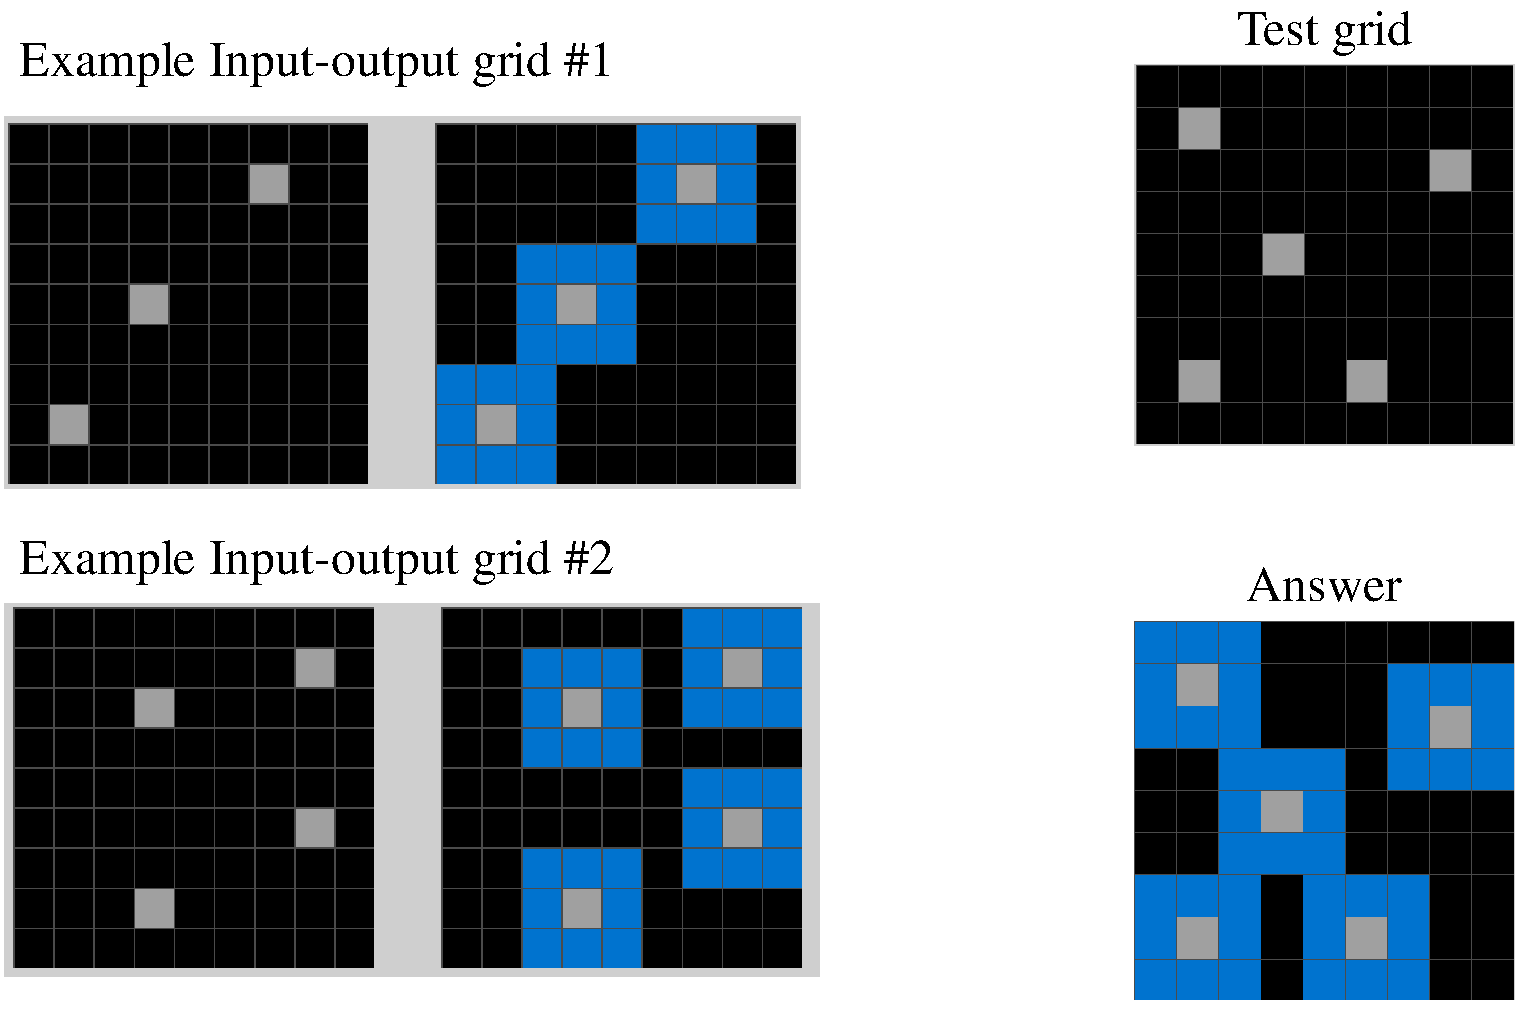
\includegraphics[width=\textwidth]{Figures/appendix/ARC_example.pdf}
    \caption{\textbf{An example task from the ARC challenge \citep{chollet2019measure}.} Given the input-output grid examples, the AI system is asked to learn the transformation rules and then apply these learned rules to the test grid to predict the final answer.}
    \label{append_fig:arc_example}
\end{figure}
\label{append_section:arc_details}



An example task from the ARC challenge is shown in \Cref{append_fig:arc_example}. 
In the ARC challenge experiments (\Cref{section:expr_arc}), we represent the grids as strings of 2-D arrays, where each color is represented by an integer. We instruct the meta agent to design agents that generate code as solutions rather than directly outputting answers. Additionally, we provide two tool functions within the framework: (1) to test whether the generated code can solve the example grids and (2) to obtain the task’s answer by applying the generated code to the test grid. The accuracy rate is calculated by the Exact Match between the reference solution and the predicted answer. The meta agent uses ``gpt-4o-2024-05-13''~\citep{openai2024gpt4}, while discovered agents and baselines are evaluated using ``gpt-3.5-turbo-0125''~\citep{openai_gpt3.5} to reduce compute cost.

The domain description of ARC for the meta agent is shown below:

\begin{mybox}{Description of ARC for the meta agent.}
\small
Your aim is to find an optimal agent performing well on the ARC (Abstraction and Reasoning Corpus) challenge. \\
In this challenge, each task consists of three demonstration examples, and one test example. Each Example consists of an “input grid” and an “output grid”. Test-takers need to use the transformation rule learned from the examples to predict the output grid for the test example.\\

\# An example task from ARC challenge:\\

\#\# Task Overview:\\
You will be given some number of paired example inputs and outputs grids. The outputs were produced by applying a transformation rule to the input grids. In addition to the paired example inputs and outputs, there is also one test input without a known output.\\
The inputs and outputs are each ``grids''. A grid is a rectangular matrix of integers between 0 and 9 (inclusive). Each number corresponds to a color. 0 is black.\\
Your task is to determine the transformation rule from examples and find out the answer, involving determining the size of the output grid for the test and correctly filling each cell of the grid with the appropriate color or number.\\

The transformation only needs to be unambiguous and applicable to the example inputs and the test input. It doesn't need to work for all possible inputs. Observe the examples carefully, imagine the grid visually, and try to find the pattern.\\

\#\# Examples:\\
\#\#\# Example 0:\\
input = [[0,0,0,0,5,0,0,0,0], [0,0,0,0,5,0,0,0,0], [0,0,0,4,5,0,0,0,0], [0,0,0,4,5,4,4,0,0], [0,0,3,3,5,0,0,0,0], [0,0,0,3,5,0,0,0,0], [0,0,0,3,5,3,3,3,0], [0,0,0,3,5,0,0,0,0], [0,0,0,0,5,0,0,0,0], [0,0,0,0,5,0,0,0,0]]\\
output = [[0,0,0,0], [0,0,0,0], [0,0,0,4], [0,0,4,4], [0,0,3,3], [0,0,0,3], [0,3,3,3], [0,0,0,3], [0,0,0,0], [0,0,0,0]]\\

\#\#\# Example 1:\\
input = [[0,0,0,0,5,0,0,0,0], [0,0,0,2,5,0,0,0,0], [0,0,0,2,5,2,6,0,0], [0,0,0,2,5,0,0,0,0], [0,0,0,2,5,2,2,2,0], [0,0,6,6,5,6,0,0,0], [0,0,0,2,5,0,0,0,0], [0,2,2,0,5,2,0,0,0], [0,0,0,2,5,0,0,0,0], [0,0,0,0,5,0,0,0,0]]\\
output = [[0,0,0,0], [0,0,0,2], [0,0,6,2], [0,0,0,2], [0,2,2,2], [0,0,6,6], [0,0,0,2], [0,2,2,2], [0,0,0,2], [0,0,0,0]]\\

\#\#\# Example 2:\\
input = [[0,0,0,0,5,0,0,0,0], [0,0,0,0,5,7,0,0,0], [0,0,0,8,5,0,0,0,0], [0,0,0,8,5,0,0,0,0], [0,7,8,8,5,0,0,0,0], [0,0,0,0,5,8,8,0,0], [0,0,0,8,5,0,0,0,0], [0,0,0,8,5,0,0,0,0], [0,0,0,0,5,8,7,0,0], [0,0,0,0,5,0,0,0,0]]\\
output= [[0,0,0,0], [0,0,0,7], [0,0,0,8], [0,0,0,8], [0,7,8,8], [0,0,8,8], [0,0,0,8], [0,0,0,8], [0,0,7,8], [0,0,0,0]]\\

\#\#\# Test Problem:\\
input = [[0,0,0,0,5,0,0,0,0], [0,0,0,1,5,0,0,0,0], [0,0,0,1,5,1,0,0,0], [0,1,1,1,5,1,1,1,6], [0,0,0,6,5,6,6,0,0], [0,0,0,0,5,1,1,1,0], [0,0,0,1,5,0,0,0,0], [0,0,0,1,5,1,6,0,0], [0,0,0,0,5,6,0,0,0], [0,0,0,0,5,0,0,0,0]]\\

Analyze the transformation rules based on the provided Examples and determine what the output should be for the Test Problem.\\
\end{mybox}

Here we present the best agent on ARC discovered by \ouralgo.

\begin{lstlisting}[style=pythonstyle, caption={The best agent on ARC discovered by \ouralgo}]
# Structured Feedback and Ensemble Agent
def forward(self, taskInfo):
    # Step 1: Generate initial candidate solutions using multiple FM Modules
    initial_instruction = 'Please think step by step and then solve the task by writing the code.'
    num_candidates = 5  # Number of initial candidates
    initial_module = [FM_Module(['thinking', 'code'], 'Initial Solution', temperature=0.8) for _ in range(num_candidates)]

    initial_solutions = []
    for i in range(num_candidates):
        thoughts = initial_module[i]([taskInfo], initial_instruction)
        thinking, code = thoughts[0], thoughts[1]
        feedback, correct_examples, wrong_examples = self.run_examples_and_get_feedback(code)
        if len(correct_examples) > 0:  # Only consider solutions that passed at least one example
            initial_solutions.append({'thinking': thinking, 'code': code, 'feedback': feedback, 'correct_count': len(correct_examples)})

    # Step 2: Simulate human-like feedback for each candidate solution
    human_like_feedback_module = FM_Module(['thinking', 'feedback'], 'Human-like Feedback', temperature=0.5)
    human_feedback_instruction = 'Please provide human-like feedback for the code, focusing on common mistakes, heuristic corrections, and best practices.'

    for sol in initial_solutions:
        thoughts = human_like_feedback_module([taskInfo, sol['thinking'], sol['code']], human_feedback_instruction)
        human_thinking, human_feedback = thoughts[0], thoughts[1]
        sol['human_feedback'] = human_feedback

    # Step 3: Assign expert advisors to evaluate and provide targeted feedback
    expert_roles = ['Efficiency Expert', 'Readability Expert', 'Simplicity Expert']
    expert_advisors = [FM_Module(['thinking', 'feedback'], role, temperature=0.6) for role in expert_roles]
    expert_instruction = 'Please evaluate the given code and provide targeted feedback for improvement.'

    for sol in initial_solutions:
        sol_feedback = {}
        for advisor in expert_advisors:
            thoughts = advisor([taskInfo, sol['thinking'], sol['code']], expert_instruction)
            thinking, feedback = thoughts[0], thoughts[1]
            sol_feedback[advisor.role] = feedback
        sol['expert_feedback'] = sol_feedback

    # Step 4: Parse and structure the feedback to avoid redundancy and refine the solutions iteratively
    max_refinement_iterations = 3
    refinement_module = FM_Module(['thinking', 'code'], 'Refinement Module', temperature=0.5)
    refined_solutions = []

    for sol in initial_solutions:
        for i in range(max_refinement_iterations):
            combined_feedback = sol['feedback'].content + sol['human_feedback'].content + ''.join([fb.content for fb in sol['expert_feedback'].values()])
            structured_feedback = ' '.join(set(combined_feedback.split()))  # Avoid redundancy
            refinement_instruction = 'Using the structured feedback, refine the solution to improve its performance.'
            thoughts = refinement_module([taskInfo, sol['thinking'], sol['code'], Info('feedback', 'Structured Feedback', structured_feedback, i)], refinement_instruction, i)
            refinement_thinking, refined_code = thoughts[0], thoughts[1]
            feedback, correct_examples, wrong_examples = self.run_examples_and_get_feedback(refined_code)
            if len(correct_examples) > 0:
                sol.update({'thinking': refinement_thinking, 'code': refined_code, 'feedback': feedback, 'correct_count': len(correct_examples)})
                refined_solutions.append(sol)

    # Step 5: Select the best-performing solutions and make a final decision using an ensemble approach
    sorted_solutions = sorted(refined_solutions, key=lambda x: x['correct_count'], reverse=True)
    top_solutions = sorted_solutions[:3]  # Select the top 3 solutions

    final_decision_instruction = 'Given all the above solutions, reason over them carefully and provide a final answer by writing the code.'
    final_decision_module = refinement_module(['thinking', 'code'], 'Final Decision Module', temperature=0.1)
    final_inputs = [taskInfo] + [item for solution in top_solutions for item in [solution['thinking'], solution['code'], solution['feedback']]]
    final_thoughts = final_decision_module(final_inputs, final_decision_instruction)
    final_thinking, final_code = final_thoughts[0], final_thoughts[1]
    answer = self.get_test_output_from_code(final_code)
    return answer
\end{lstlisting}

\section{Experiment Details for Reasoning and Problem-Solving Domains}
\label{append_section:extensive_domains_details}

To reduce costs during search and evaluation, we sample subsets of data from each domain. For GPQA (Science), we use GPQA\_diamond and the validation set consists of 32 questions, while the remaining 166 questions form the test set. For the other domains, the validation and test sets are sampled with 128 and 800 questions, respectively. We evaluate agents five times for GPQA and once for the other domains to maintain a consistent total number of evaluations. Each domain uses zero-shot style questions, except DROP (Reading Comprehension), which uses one-shot style questions following the practice in \citep{simple_evals}. The meta agent uses ``gpt-4o-2024-05-13''~\citep{openai2024gpt4}, while discovered agents and baselines are evaluated using ``gpt-3.5-turbo-0125''~\citep{openai_gpt3.5} to reduce compute cost.

We present the description of each domain we provide to the meta agent. 

\begin{mybox}{Description of DROP (Reading Comprehension).}
\small
Your aim is to find an optimal agent performing well on the Reading Comprehension Benchmark Requiring Discrete Reasoning Over Paragraphs (DROP), which assesses the ability to perform discrete reasoning and comprehend detailed information across multiple paragraphs.\\

\#\# An example question from DROP:\\

You will be asked to read a passage and answer a question.\\ \\
Passage:\\
Non-nationals make up more than half of the population of Bahrain, with immigrants making up about 55\% of the overall population.  Of those, the vast majority come from South and Southeast Asia: according to various media reports and government statistics dated between 2005-2009 roughly 290,000 Indians, 125,000 Bangladeshis, 45,000 Pakistanis, 45,000 Filipinos, and 8,000 Indonesians.\\ \\
Question: What two nationalities had the same number of people living in Bahrain between 2005-2009?\\
Answer [Not Given]: Pakistanis and Filipinos
\end{mybox}

\begin{mybox}{Description of GPQA (Science) for the meta agent.}
\small
Your aim is to find an optimal agent performing well on the GPQA (Graduate-Level Google-Proof Q\&A Benchmark). This benchmark consists of challenging multiple-choice questions across the domains of biology, physics, and chemistry, designed by domain experts to ensure high quality and difficulty.\\

\#\# An example question from GPQA:\\

Two quantum states with energies E1 and E2 have a lifetime of $10^-9$ sec and $10^-8$ sec, respectively. We want to clearly distinguish these two energy levels. Which one of the following options could be their energy difference so that they be clearly resolved?\\

Answer choices:\\
$10^-9$ eV\\
$10^-8$ eV\\
$10^-7$ eV\\
$10^-6$ eV\\

Correct answer [Not provided]:\\
$10^-7$ eV\\

Explanation [Not provided]:\\
According to the uncertainty principle, Delta E* Delta t=hbar/2. Delta t is the lifetime and Delta E is the width of the energy level. With Delta t=$10^-9$ s==$>$ Delta E1= 3.3 $10^-7$ ev. And Delta t=$10^-11$ s gives Delta E2=$3.310^-8$ eV.
Therefore, the energy difference between the two states must be significantly greater than $10^-7$ ev. So the answer is $10^-4$ ev.
\end{mybox}

\begin{mybox}{Description of MGSM (Math) for the meta agent.}
\small
Your aim is to find an optimal agent performing well on the Multilingual Grade School Math Benchmark (MGSM) which evaluates mathematical problem-solving abilities across various languages to ensure broad and effective multilingual performance.\\

\#\# An example question from MGSM:\\

\begin{CJK}{UTF8}{min}
**Question**: この数学の問題を解いてください。\\

近所では、ペットのウサギの数がペットの犬と猫を合わせた数よりも12匹少ない。犬1匹あたり2匹の猫がおり、犬の数は60匹だとすると、全部で近所には何匹のペットがいますか？\\
\end{CJK}

**Answer (Not Given)**: 348
\end{mybox}

\begin{mybox}{Description of MMLU (Mult-task) for the meta agent.}
\small
Your aim is to find an optimal agent performing well on the MMLU (Massive Multitask Language Understanding) benchmark, a challenging evaluation that assesses a model's ability to answer questions across a wide range of subjects and difficulty levels. It includes subjects from STEM, social sciences, humanities, and more.\\

\#\# An example question from MMLU:\\

Answer the following multiple-choice question.\\

The constellation ... is a bright W-shaped constellation in the northern sky.\\

(A) Centaurus\\
(B) Cygnus\\
(C) Cassiopeia\\
(D) Cepheus\\

\end{mybox}

\section{Baselines}
\label{append_section:baselines}

In this paper, we implement five state-of-the-art hand-designed agent baselines for experiments on ARC (\Cref{section:expr_arc}): (1) Chain-of-Thought (COT) \citep{wei2022chain}, (2) Self-Consistency with Chain-of-Thought (COT-SC)\citep{wang2023selfconsistency}, (3) Self-Refine~\citep{madaan2024self,shinn2024reflexion}, (4) LLM-Debate~\citep{du2023improving}, and (5) Quality-Diversity, a simplified version of Intelligent Go-Explore~\citep{lu2024intelligent}.

In addition to these baselines, we implement two more for experiments on Reasoning and Problem-Solving domains (\Cref{section:expr_four_main_domains}): (6) Step-back Abstraction~\citep{zheng2023stepback} and (7) Role Assignment \citep{xu2023expertprompting}. An example implementation of Self-Refine with our simple framework is shown in \Cref{append_section:utility_codes}.

In COT, we prompt the FM to think step by step before answering the question. In COT-SC, we sample $N=5$ answers and then perform an ensemble using either majority voting or an FM query. In Self-Refine, we allow up to five refinement iterations, with an early stop if the critic deems the answer correct. In LLM-Debate, each debate module is assigned a unique role, such as Physics Expert or Chemistry Expert, and the debate lasts for two rounds. In Quality-Diversity, we conduct three iterations to collect diverse answers based on previously proposed ones. In Role Assignment, we use an FM query to first choose a role from a predefined set, and then use another FM query to answer the question by acting within the chosen role.

\section{Example Agents}
\label{append_section:example_agents}

In this section, we present the detailed implementation of three example discovered agents by \ouralgo shown in \Cref{fig:algo}. The ``Multi-Step Peer Review Agent'' and ``Divide and Conquer Agent'' were discovered during the search in the Reading Comprehension domain (GPQA) \citep{rein2023gpqa}, while the ``Verified Multimodal Agent'' was discovered during the search in the Math domain (MGSM) \citep{shi2023language}.

\begin{lstlisting}[style=pythonstyle, caption={Example discovered agent: Multi-Step Peer Review Agent}]
def forward(self, taskInfo):
    initial_instruction = "Please think step by step and then solve the task."
    critique_instruction = "Please review the answer above and provide feedback on where it might be wrong. If you are absolutely sure it is correct, output 'True' in 'correct'."
    refine_instruction = "Given previous attempts and feedback, carefully consider where you could go wrong in your latest attempt. Using insights from previous attempts, try to solve the task better."
    final_decision_instruction = "Given all the above thinking and answers, reason over them carefully and provide a final answer."

    FM_modules = [FM_module(['thinking', 'answer'], 'FM Module', role=role) for role in ['Physics Expert', 'Chemistry Expert', 'Biology Expert', 'Science Generalist']]
    critic_modules = [FM_module(['feedback', 'correct'], 'Critic', role=role) for role in ['Physics Critic', 'Chemistry Critic', 'Biology Critic', 'General Critic']]
    final_decision_module = FM_module(['thinking', 'answer'], 'Final Decision', temperature=0.1)

    all_thinking = [[] for _ in range(len(FM_modules))]
    all_answer = [[] for _ in range(len(FM_modules))]
    all_feedback = [[] for _ in range(len(FM_modules))]

    for i in range(len(FM_modules)):
        thinking, answer = FM_modules[i]([taskInfo], initial_instruction)
        all_thinking[i].append(thinking)
        all_answer[i].append(answer)

    for i in range(len(FM_modules)):
        for j in range(len(FM_modules)):
            if i != j:
                feedback, correct = critic_modules[j]([taskInfo, all_thinking[i][0], all_answer[i][0]], critique_instruction)
                all_feedback[i].append(feedback)

    for i in range(len(FM_modules)):
        refine_inputs = [taskInfo, all_thinking[i][0], all_answer[i][0]] + all_feedback[i]
        thinking, answer = FM_modules[i](refine_inputs, refine_instruction)
        all_thinking[i].append(thinking)
        all_answer[i].append(answer)

    final_inputs = [taskInfo] + [all_thinking[i][1] for i in range(len(FM_modules))] + [all_answer[i][1] for i in range(len(FM_modules))]
    thinking, answer = final_decision_module(final_inputs, final_decision_instruction)

    return answer
\end{lstlisting}


\begin{lstlisting}[style=pythonstyle, caption={Example discovered agent: Divide and Conquer Agent}]
def forward(self, taskInfo):
    # Step 1: Decompose the problem into sub-problems
    decomposition_instruction = "Please decompose the problem into smaller, manageable sub-problems. List each sub-problem clearly."
    decomposition_module = FM_Module(['thinking', 'sub_problems'], 'Decomposition Module')

    # Step 2: Assign each sub-problem to a specialized expert
    sub_problem_instruction = "Please think step by step and then solve the sub-problem."
    specialized_experts = [FM_Module(['thinking', 'sub_solution'], 'Specialized Expert', role=role) for role in ['Physics Expert', 'Chemistry Expert', 'Biology Expert', 'General Expert']]

    # Step 3: Integrate the sub-problem solutions into the final answer
    integration_instruction = "Given the solutions to the sub-problems, integrate them to provide a final answer to the original problem."
    integration_module = FM_Module(['thinking', 'answer'], 'Integration Module', temperature=0.1)

    # Decompose the problem
    thinking, sub_problems = decomposition_module([taskInfo], decomposition_instruction)

    # Ensure sub_problems is a string and split into individual sub-problems
    sub_problems_list = sub_problems.content.split('\n') if isinstance(sub_problems.content, str) else []

    # Solve each sub-problem
    sub_solutions = []
    for i, sub_problem in enumerate(sub_problems_list):
        sub_problem_info = Info('sub_problem', decomposition_module.__repr__(), sub_problem, i)
        sub_thinking, sub_solution = specialized_experts[i % len(specialized_experts)]([sub_problem_info], sub_problem_instruction)
        sub_solutions.append(sub_solution)

    # Integrate the sub-problem solutions
    integration_inputs = [taskInfo] + sub_solutions
    thinking, answer = integration_module(integration_inputs, integration_instruction)

    return answer
\end{lstlisting}

\begin{lstlisting}[style=pythonstyle, caption={Example discovered agent: Verified Multimodal Agent}]
def forward(self, taskInfo):
    # Instruction for generating visual representation of the problem
    visual_instruction = "Please create a visual representation (e.g., diagram, graph) of the given problem."
    
    # Instruction for verifying the visual representation
    verification_instruction = "Please verify the accuracy and relevance of the visual representation. Provide feedback and suggestions for improvement if necessary."
    
    # Instruction for solving the problem using the verified visual aid
    cot_instruction = "Using the provided visual representation, think step by step and solve the problem."
    
    # Instantiate the visual representation module, verification module, and Chain-of-Thought module
    visual_module = FM_Module(['visual'], 'Visual Representation Module')
    verification_module = FM_Module(['feedback', 'verified_visual'], 'Verification Module')
    cot_module = FM_Module(['thinking', 'answer'], 'Chain-of-Thought Module')
    
    # Generate the visual representation of the problem
    visual_output = visual_module([taskInfo], visual_instruction)
    visual_representation = visual_output[0]  # Using Info object directly
    
    # Verify the visual representation
    feedback, verified_visual = verification_module([taskInfo, visual_representation], verification_instruction)
    
    # Use the verified visual representation to solve the problem
    thinking, answer = cot_module([taskInfo, verified_visual], cot_instruction)
    return answer
\end{lstlisting}


\section{Pseudocode of the Meta Agent Search}

\label{append_section:pseudocode}
In this section, we provide the pseudocode for the Meta Agent Search algorithm to clarify its implementation and workflow. The pseudocode outlines the iterative process of designing, evaluating, and refining agents using a meta agent, as described in the main text.


\begin{algorithm}[H]
\caption{Meta Agent Search Algorithm}
\label{alg:meta_agent_search}
\begin{algorithmic}[1]
\State \textbf{Input:} Target domain validation data, maximum iterations $N$
\State \textbf{Output:} Archive of discovered agents
\State Initialize archive $\mathcal{A}$ with baseline agents (e.g., Chain-of-Thought, Self-Refine)

\For{$i = 1$ to $N$}
    \State \textbf{Design Step:} Meta agent generates a new agent:
    \State \quad (a) Outputs design reasoning
    \State \quad (b) Implements the design in code
    \State \quad (c) Performs two self-reflection steps to ensure novelty and correctness
    \State \textbf{Evaluation Step:} Evaluate the new agent on target domain validation data:
    \State \quad (a) If the agent produces errors during evaluation, refine the design up to 5 iterations
    \State \quad (b) Re-run the evaluation after each refinement
    \State \textbf{Update Step:} Add the refined agent and its evaluation metrics to the archive $\mathcal{A}$
\EndFor

\State \textbf{Return:} Final archive $\mathcal{A}$
\end{algorithmic}
\end{algorithm}

\section{Impact of Initialization}
\label{append_sec:init}

One of the key claims of our work is that the \textit{code space} representation allows for better utilization of existing human efforts (\Cref{section:problem_formulation}), enabling a more efficient search process than starting entirely from scratch. To further investigate the effects of initialization, we conducted experiments where the Meta Agent Search algorithm was run without any initial agent designs, contrasting with our standard approach that incorporates human-designed solutions into the search process.

The results, presented in Table~\ref{tab:empty_init}, demonstrate that even without initial agent designs, Meta Agent Search discovers agents that outperform all hand-crafted baselines across all evaluated domains. This finding underscores the robustness of our method, as it effectively leverages the inherent structure of the code space to explore and optimize agent designs.

Interestingly, while the inclusion of good initial solutions generally leads to improved performance, the math domain exhibited a unique outcome: starting from scratch resulted in superior performance. We hypothesize that the absence of predefined design patterns in this case encouraged a broader and more diverse exploration of reasoning strategies within the limited number of iterations. Such diversity appears particularly beneficial for math tasks, which demand flexible and varied approaches to reasoning.

This observation opens up an intriguing avenue for future research: exploring how the choice and quality of initialization impact search effectiveness across different domains. For instance, it would be valuable to identify conditions under which starting without initial solutions may yield performance gains, or to design strategies that combine the advantages of both initialization and broad exploration.

\begin{table}[h]
    \centering
    
    \caption{\textbf{Performance comparison of Meta Agent Search with and without initial agent designs across multiple domains.} The results show that even without initialization, Meta Agent Search outperforms hand-designed baselines in all domains. However, incorporating initial solutions generally leads to better performance, except in the math domain, where starting without initialization yields superior results.}
    \resizebox{\textwidth}{!}{ % Resize table to fit the width
    \begin{tabular}{>{\raggedright}p{6cm}cccc}
        \toprule
        \multirow{2}{*}{\textbf{Agent Name}} & \multicolumn{1}{c}{\textbf{F1 Score}} & \multicolumn{3}{c}{\textbf{Accuracy (\%)}} \\
        \cmidrule(lr){2-2}\cmidrule(lr){3-5}
        & \textbf{Reading Comprehension} & \textbf{Math}  & \textbf{Multi-task} & \textbf{Science} \\
        \midrule
        \rowcolor{gray!20} \multicolumn{5}{>{\centering\arraybackslash}p{16.3cm}}{\textbf{State-of-the-art Hand-designed Agents}} \vspace{0.1cm} \\ 
        Chain-of-Thought~\citep{wei2022chain} & \rule{0pt}{2.2ex}$64.2 \pm 0.9$ & $28.0 \pm 3.1$ & $65.4 \pm 3.3$ & $29.2 \pm 3.1$ \\
        COT-SC~\citep{wang2023selfconsistency} & \rule{0pt}{2.2ex}$64.4 \pm 0.8$ & $28.2 \pm 3.1$ & $65.9 \pm 3.2$ & $30.5 \pm 3.2$ \\
        Self-Refine~\citep{madaan2024self} & \rule{0pt}{2.2ex}$59.2 \pm 0.9$ & $27.5 \pm 3.1$ & $63.5 \pm 3.4$ & $\mathbf{31.6 \pm 3.2}$ \\
        LLM Debate~\citep{du2023improving} & \rule{0pt}{2.2ex}$60.6 \pm 0.9$ & $39.0 \pm 3.4$ & $65.6 \pm 3.3$ & $\mathbf{31.4 \pm 3.2}$ \\
        Step-back Abstraction~\citep{zheng2023stepback} & \rule{0pt}{2.2ex}$60.4 \pm 1.0$ & $31.1 \pm 3.2$ & $65.1 \pm 3.3$ & $26.9 \pm 3.0$ \\
        Quality-Diversity~\citep{lu2024intelligent} & \rule{0pt}{2.2ex}$61.8 \pm 0.9$ & $23.8 \pm 3.0$ & $65.1 \pm 3.3$ & $30.2 \pm 3.1$ \\
        Role Assignment~\citep{xu2023expertprompting} & \rule{0pt}{2.2ex}$65.8 \pm 0.9$ & $30.1 \pm 3.2$ & $64.5 \pm 3.3$ & $31.1 \pm 3.1$ \\
        % Add more rows here as needed
        \midrule
        \rowcolor{gray!20} \multicolumn{5}{>{\centering\arraybackslash}p{16.3cm}}{\textbf{\problemlong on Different Domains}} \vspace{0.1cm} \\
        Meta Agent Search (Empty Initialization) & \rule{0pt}{2.2ex}$73.9 \pm 0.9$ & $\mathbf{67.5 \pm 3.3}$ & $\mathbf{68.5 \pm 3.3}$ & $\mathbf{32.7 \pm 3.2}$ \\
        Meta Agent Search & \rule{0pt}{2.2ex}$\mathbf{79.4 \pm 0.8}$ & $53.4 \pm 3.5$ & $\mathbf{69.6 \pm 3.2}$ & $\mathbf{34.6 \pm 3.2}$ \\
        \bottomrule
    \end{tabular}}
    \label{tab:empty_init}
    % \vspace{-0.5cm}
\end{table}

\section{Cost of Experiments}
\label{append_section:cost}

A single run of search and evaluation on ARC (\Cref{section:expr_arc}) costs approximately \$500 USD in OpenAI API costs, while a run within the reasoning and problem-solving domains (\Cref{section:expr_four_main_domains}) costs about \$300 USD.

The primary expense comes from querying the ``gpt-3.5-turbo-0125'' model during the evaluation of discovered agents.
Notably, the latest GPT-4 model, ``gpt-4o-mini,'' is less than one-third the price of ``gpt-3.5-turbo-0125'' and offers better performance, suggesting that we could achieve improved results with \ouralgo at just one-third of the cost. Additionally, as discussed in \Cref{section:future_work}, the current naive evaluation function is both expensive and overlooks valuable information. We anticipate that future work adopting more sophisticated evaluation functions could significantly reduce the cost of \problem algorithms.
